\section{E-Mail Template of the Awareness Part}
\label{a:mail}
\lstset{language=html}
\begin{lstlisting}
<html>
  <head>
    <title>Anti Phishing Education</title>
  </head>
  <body>
    <p>Dies ist eine automatisch generierte E-Mail im Rahmen einer Anti-Phishing Education App. Falls diese nicht angefordert wurde, bitte ignorieren.</p>
    <p>Ansonsten geht es hier weiter:</p>
    <p>Wie du im Absender siehst, hast du dir gerade selbst eine E-Mail mit gefälschtem Absender geschickt. Hier ist außerdem dein Freitext:</p>
    <p>{$usermessage}</p>
    <p>Für einen Angreifer ist es ebenso einfach automatisierte E-Mails mit gefälschtem Absender und Inhalt zu verschicken. Meist enthalten diese einen Link zu einer Webseite, genau wie diese E-Mail.</p>
    <p>Um mit der App fortzufahren, klicke auf den folgenden Link.</p>
    <p><a href="http://pages.no-phish.de/maillink.php">http://www.google.com</a></p>
    <p>Viele Grüße,</p>
    <p>Dein NoPhish Team</p>
  </body>
</html>
\end{lstlisting}

%===========================================
\section{URL Generation Process}
\label{s:url_generation}
%===========================================
When playing the app (level 2-9) the user has to categorize a given URL as a phish or valid URL.
We decided against a fixed set of examples for the URLs because depending on the set size it might happen that a user keeps being confronted with the same URLs.
We believe it is essential for the user to be faced with as many different URL examples as possible.
Therefore, we decided to generate the URLs rather than composing a fixed list.
Next, we lay out the URL generation process and cover further interesting aspects of the URL generation in the subsequent sections.
\subsection{Derive Phishing URLs from Valid Example URLs}
To present attacked URLs to the user we found it most realistic to take valid URLs and apply the covered attacks to them.
For this purpose, we needed a set of valid URLs.
To build this set we used Alexa~\cite{alexa} to select various domains from the top 100 website vendors of Germany.
Then, we visited each of these websites, navigated through them and picked about 3-6 URLs for each domain we had previously selected.
We strived to balance the number of short and long URLs.
Given a list of valid URLs an attack can be applied whenever required.
In the following we discuss how this is accomplished in our implementation.
\begin{description}[leftmargin=0cm]
\item[Generate a List of Attacks for Each Level:] When starting a new level we generate a list of attacks with which the user needs to be confronted.
\item[Select a Valid URL:] Whenever a new URL is to be shown to the user we first randomly select a valid URL from the aforementioned set.
\item[Modify Valid URLs with a Generator:] Then we apply a generator to the URL that does not invalidate the URL but modifies it (cf. \autoref{s:apply_generator}).
\item[Apply an Attack:] After that we select a random attack from the previously built list and apply it to the selected valid URL.
\item[Repeat in Case Attack was not Possible:] In some cases applying a specific attack to a given URL is not possible. For example, in homograph attacks the replacement of an ``i'' with another letter in a URL which does not contain an ``i'' will fail. In these situations we have to retry.
\end{description}

\subsection{Number of Phishes and Repetitions per Level}
%\textbf{Was zur historie?}
The types of spoofed URLs the user is faced with depends on the level.
Each level introduces one ore more attacks.
The introduced attacks of each level are layed out in \autoref{s:knowledgetransferperlevel}.
In general, the URLs of each level $n$ are distributed as follows:
\begin{table}[hHtbp]
\centering
\begin{tabular}{|llll|}
\hline
Total number of URLs&$u$&$6+2*n$&Starting with 6 URLs each level has 2 more URLS.\\
Number of phishes&$p$&$u/2$&Half of the URLs are phishes.\\
Number of repetitions&$r$&$\left\lfloor p/2 \right\rfloor$&Half of the phishes are repetitions.\\
\hline
\end{tabular}
\caption{Distribution of URLs per level}
\label{t:levelurls}
\end{table}
Repetitions are also included into the list of attacks to be applied which is created upon start of each level.
The list of repetitions is filled up as follows: every level has exact one attack repetetion for each previous level. The rest of the repetitions is filled up randomly. This way, we assure that at least one example of each previous level is represented by the attack repetitions. All remaining phishes are new attacks.
There are two main exception to these rules:
\begin{description}[leftmargin=0cm]
\item[Level 1:] In level 1 the user is only confronted with valid URLs and has to select the domain.
To prevent the user from getting bored we only present 5 URLs in this level.
None of them is a phish.
\item[Level 1+2:] The first level that contains repetitions is level 3 because level 2 introduces the very first spoofing attack. Consequently, level 1 and level 2 do not have repetitions.
\end{description}

%The generated list of attacks also contains a special attack that does no real attack. This is to %simplify the URL generation. When we generated the list of attacks we save it for later reference.

\subsection{Modify Valid URLs with a Generator}
\label{s:apply_generator}
We were unsure whether we had collected sufficient valid URLs.
 For this reasons, we prepared a way to automatically modify the URLs in such a way that they remained valid URLs. 
Some ideas were to add subdomains or path strings to the URL. Queries or fragments would also  be possible. 
Later we found out that it was currently not required to implement such generators since our set contained enough URL examples. 
Yet, if we should realize in future that these URLs are not enough we have this scheme in place.
\subsection{Re-Apply an Attack in Case of Wrong User Answer}
After generating a valid URL we choose a random attack from the previously built set of attacks and apply it to the URL. We also store which attack we currently apply. This is important in case  the user fails to give a correct answer to the current URL. In this situation we will simply readd this attack to the set of attacks.
This way, we assure that the attack, which the user failed to identify, is repeated later in this level.
%\subsection{Repeat in Case Attack was not Possible}
%There are combinations of base-URL and attack where the attack doe's not alter the URL.
%Therefore it would be impossible for the user to detect the Attack and he will be confused and %might stop using the app.
%In this situation we repeat the whole URL generation process until we find a matching URL.

\section{Questionnaire of Study for Input}
\label{s:presurvey_form}
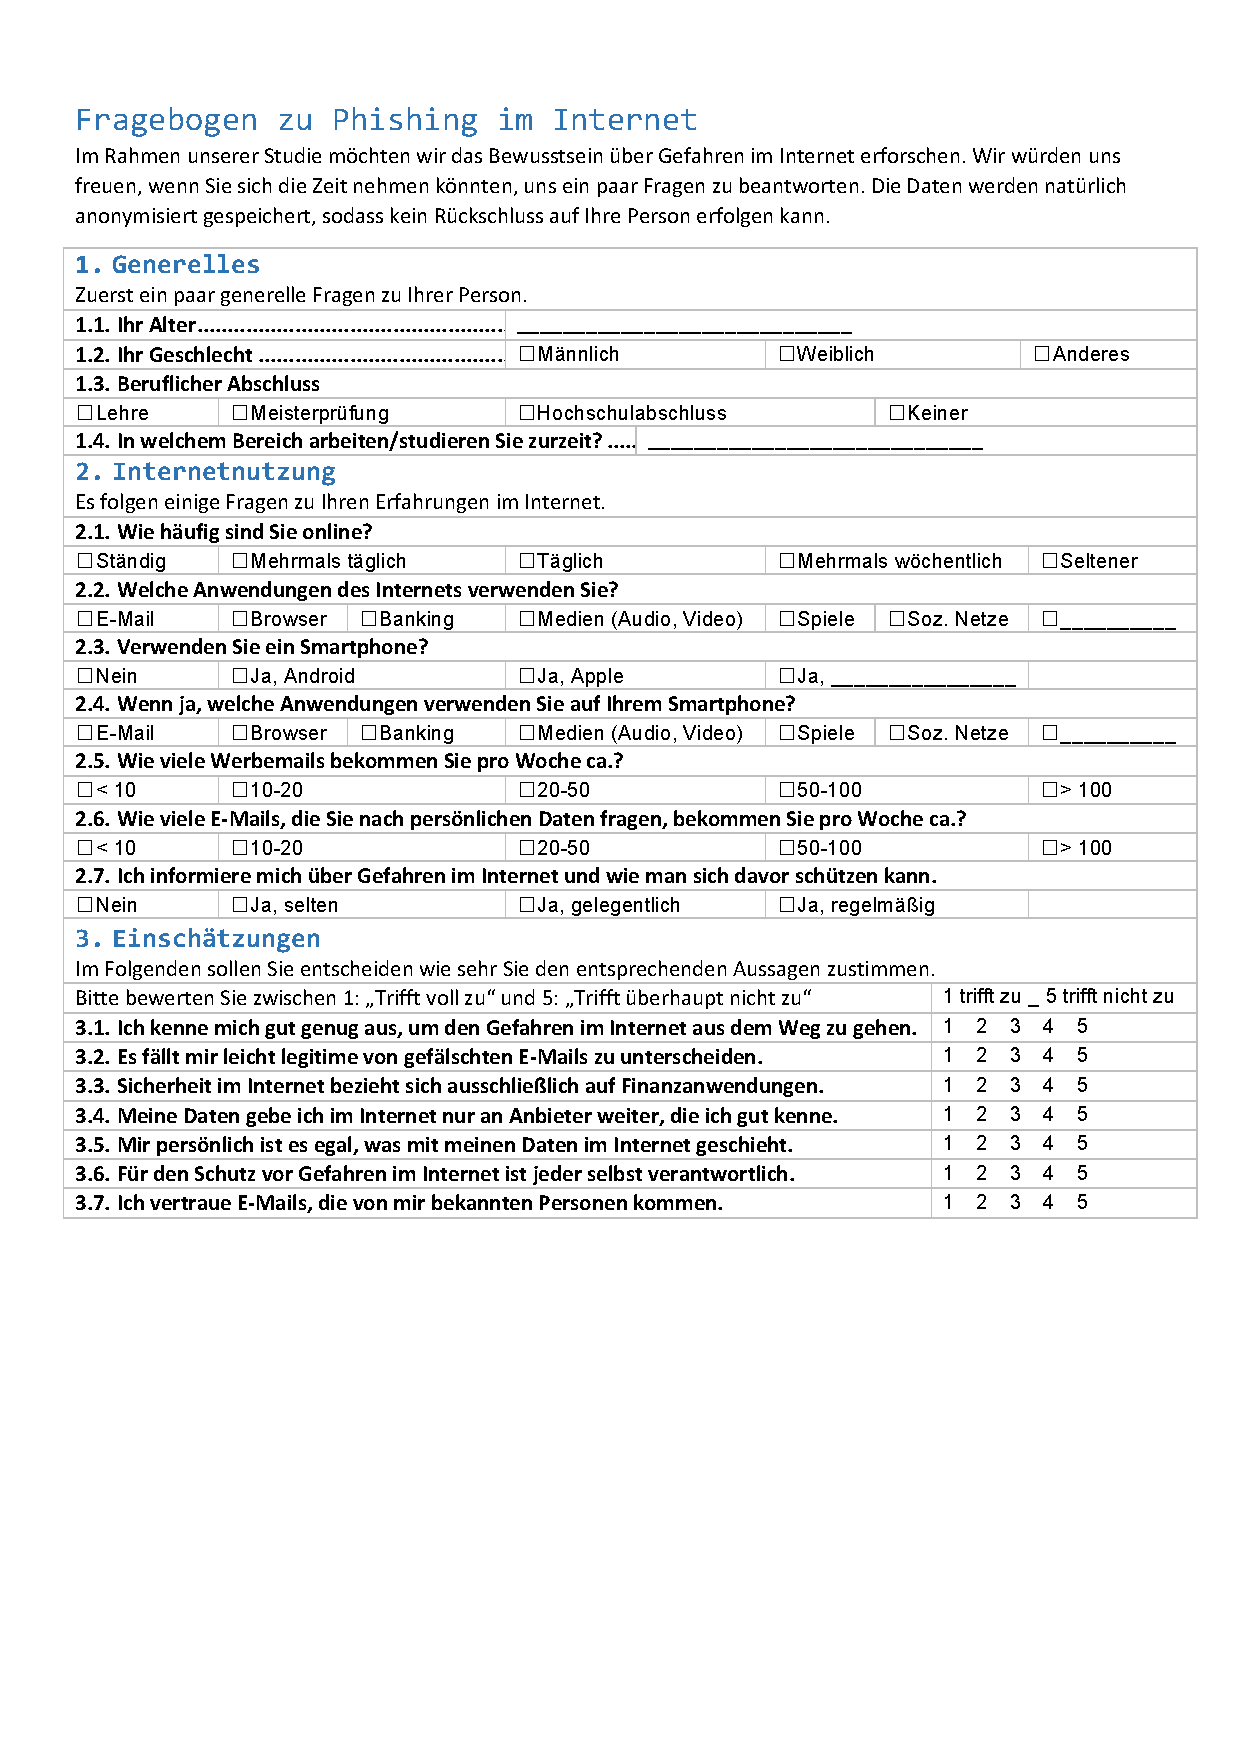
\includepdf[pages=-,frame,scale=0.8]{graphix/presurvey.pdf}


\section{Participant Recruitment for Final User Study}
\label{s:participant_recruitment_texts}

Sehr geehrte/r ....,
\newline
\newline
wir, Clemens Bergmann und Gamze Canova, sind Studenten des Fachbereichs Informatik an der TU Darmstadt und arbeiten zur Zeit unserer Masterthesis zum Thema Internetsicherheit.
\newline
\newline
Nun sind wir an dem Punkt angekommen, an dem wir eine Benutzerstudie (6.1.-11.1.2014) durchf\"{u}hren m\"{u}ssen, f\"{u}r die wir Teilnehmer suchen. Wir w\"{u}rden uns sehr freuen, wenn Sie uns hierbei unterst\"{u}tzen k\"{o}nnten. W\"{a}re es m\"{o}glich, den angeh\"{a}ngten Flyer mit dem unten stehenden Anschreiben, an Ihre StudentInnen und/oder Wissenschaftliche MitarbeiterInnen  weiterzuleiten? Wir wissen, dass es schwierig sein k\"{o}nnte potentielle Teilnehmer kurz vor Weihnachten zu erreichen, jedoch k\"{o}nnen wir jede Unterst\"{u}tzung gebrauchen und w\"{u}rden uns \"{u}ber diese sehr freuen.
\newline
\newline
Wir bedanken uns im Voraus herzlich f\"{u}r Ihre Bem\"{u}hungen und w\"{u}nschen Ihnen erholsame und besinnliche Festtage.
\newline
\newline
Mit freundlichen Gr\"{u}{\ss}en, \newline
Clemens Bergmann und Gamze Canova
\newline
\newline
Text f\"{u}r Weiterleitung:
Im Rahmen unserer Masterarbeit haben wir eine Spiele-App entwickelt, die fachfremde Benutzer \"{u}ber Internetsicherheit informiert.  Diese App soll im Rahmen einer Benutzerstudie getestet werden. Hierzu brauchen wir deine Hilfe. Die Studie wird in Gruppen zu ca. 5 Personen in der zweiten Januarwoche (6.-10.) in Darmstadt stattfinden und insgesamt ca. 90 Minuten in Anspruch nehmen.  Der/Die Beste der Gruppe gewinnt einen Amazon-Gutschein im Wert von 20\euro.  Einzige Voraussetzung f\"{u}r die Teilnahme ist, dass du Erfahrung mit der Benutzung eines Smartphones hast. Bei Interesse oder Fragen erreicht ihr uns unter netstudy@cased.de. 



\includepdf[pages={1},frame,scale=0.8]{graphix/flyer.pdf}

\section{Study Forms}
The following pages contain the forms as we used them in the user study. We did not include all example URL but only one exemplary page with an attacked URL.
\label{s:before_survey}
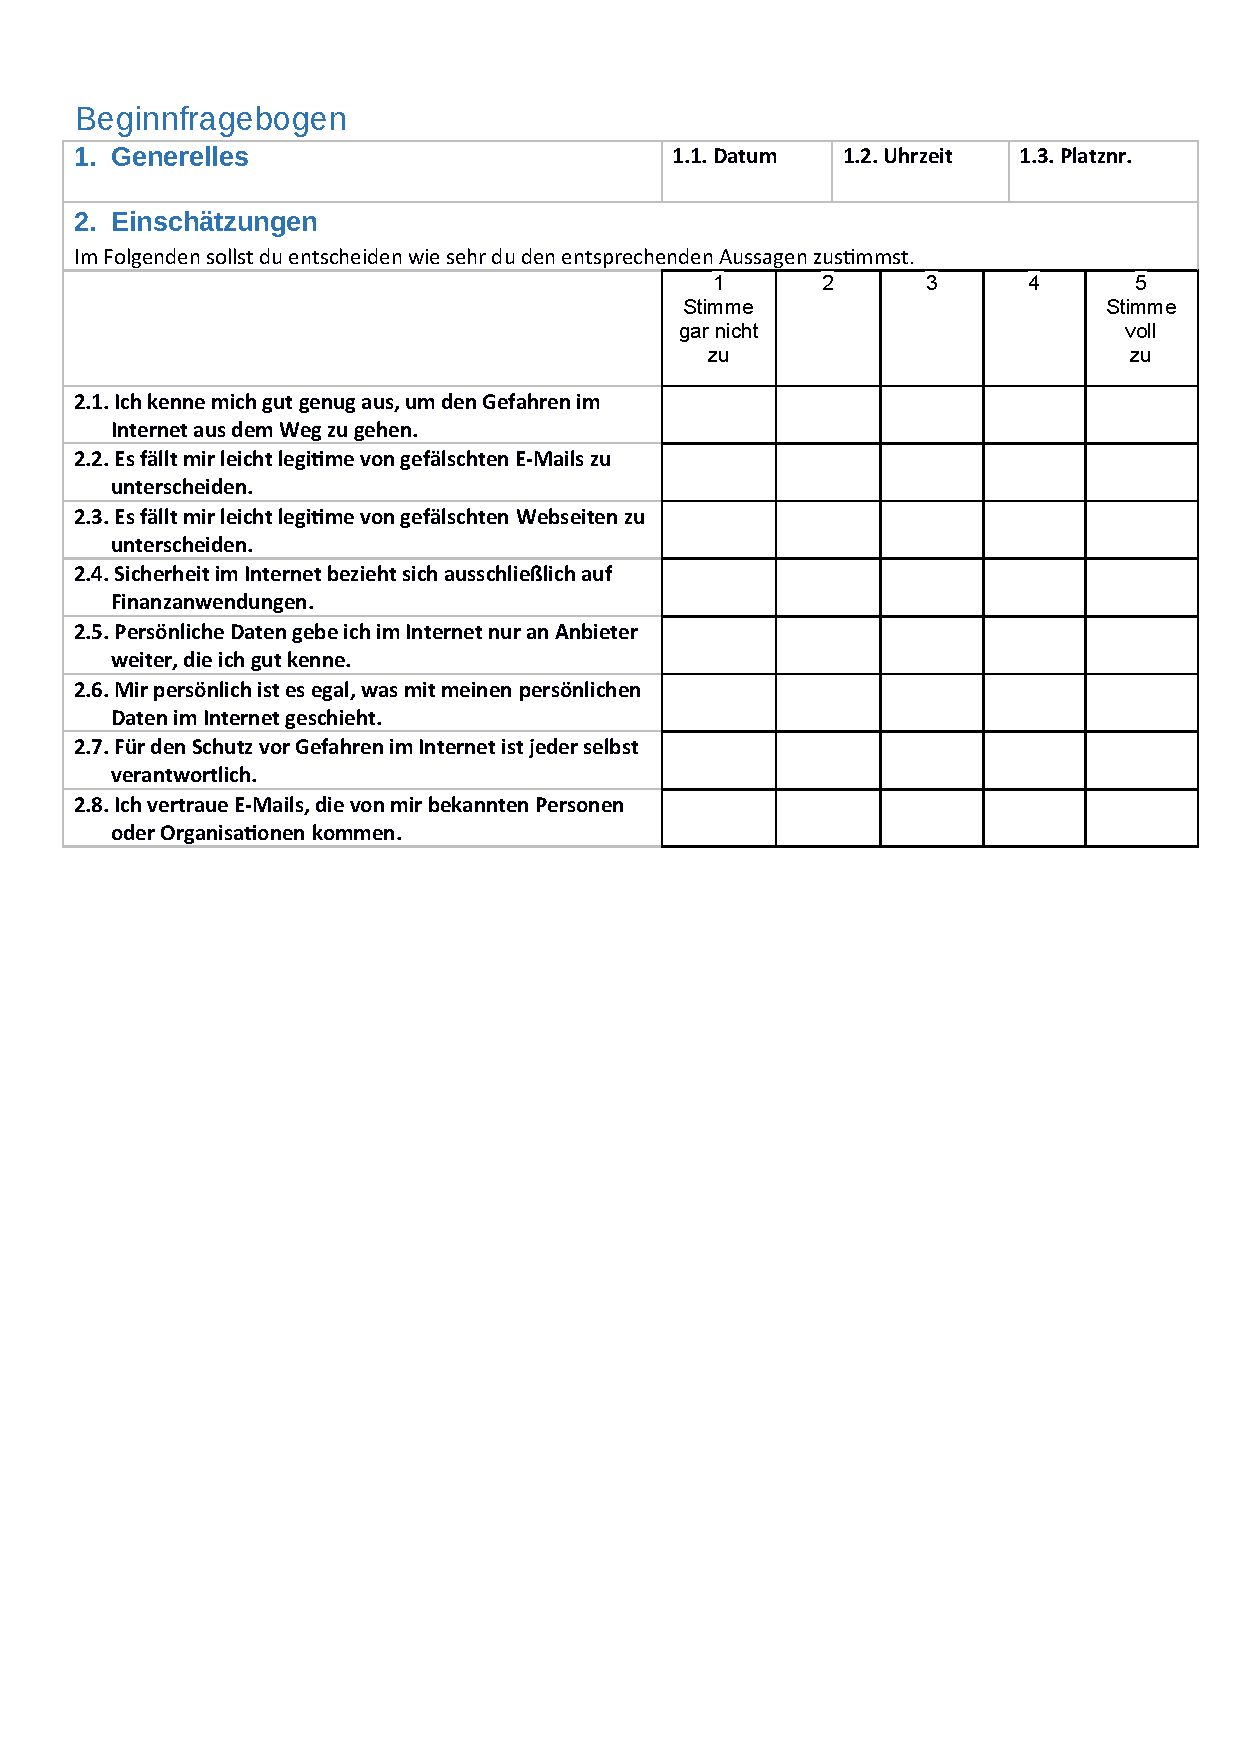
\includepdf[pages=-,frame,scale=0.8]{graphix/before_survey.pdf}
\label{s:url_survey}
\includepdf[pages={1,10},frame,scale=0.8]{graphix/url_survey.pdf}
\label{s:after_survey}
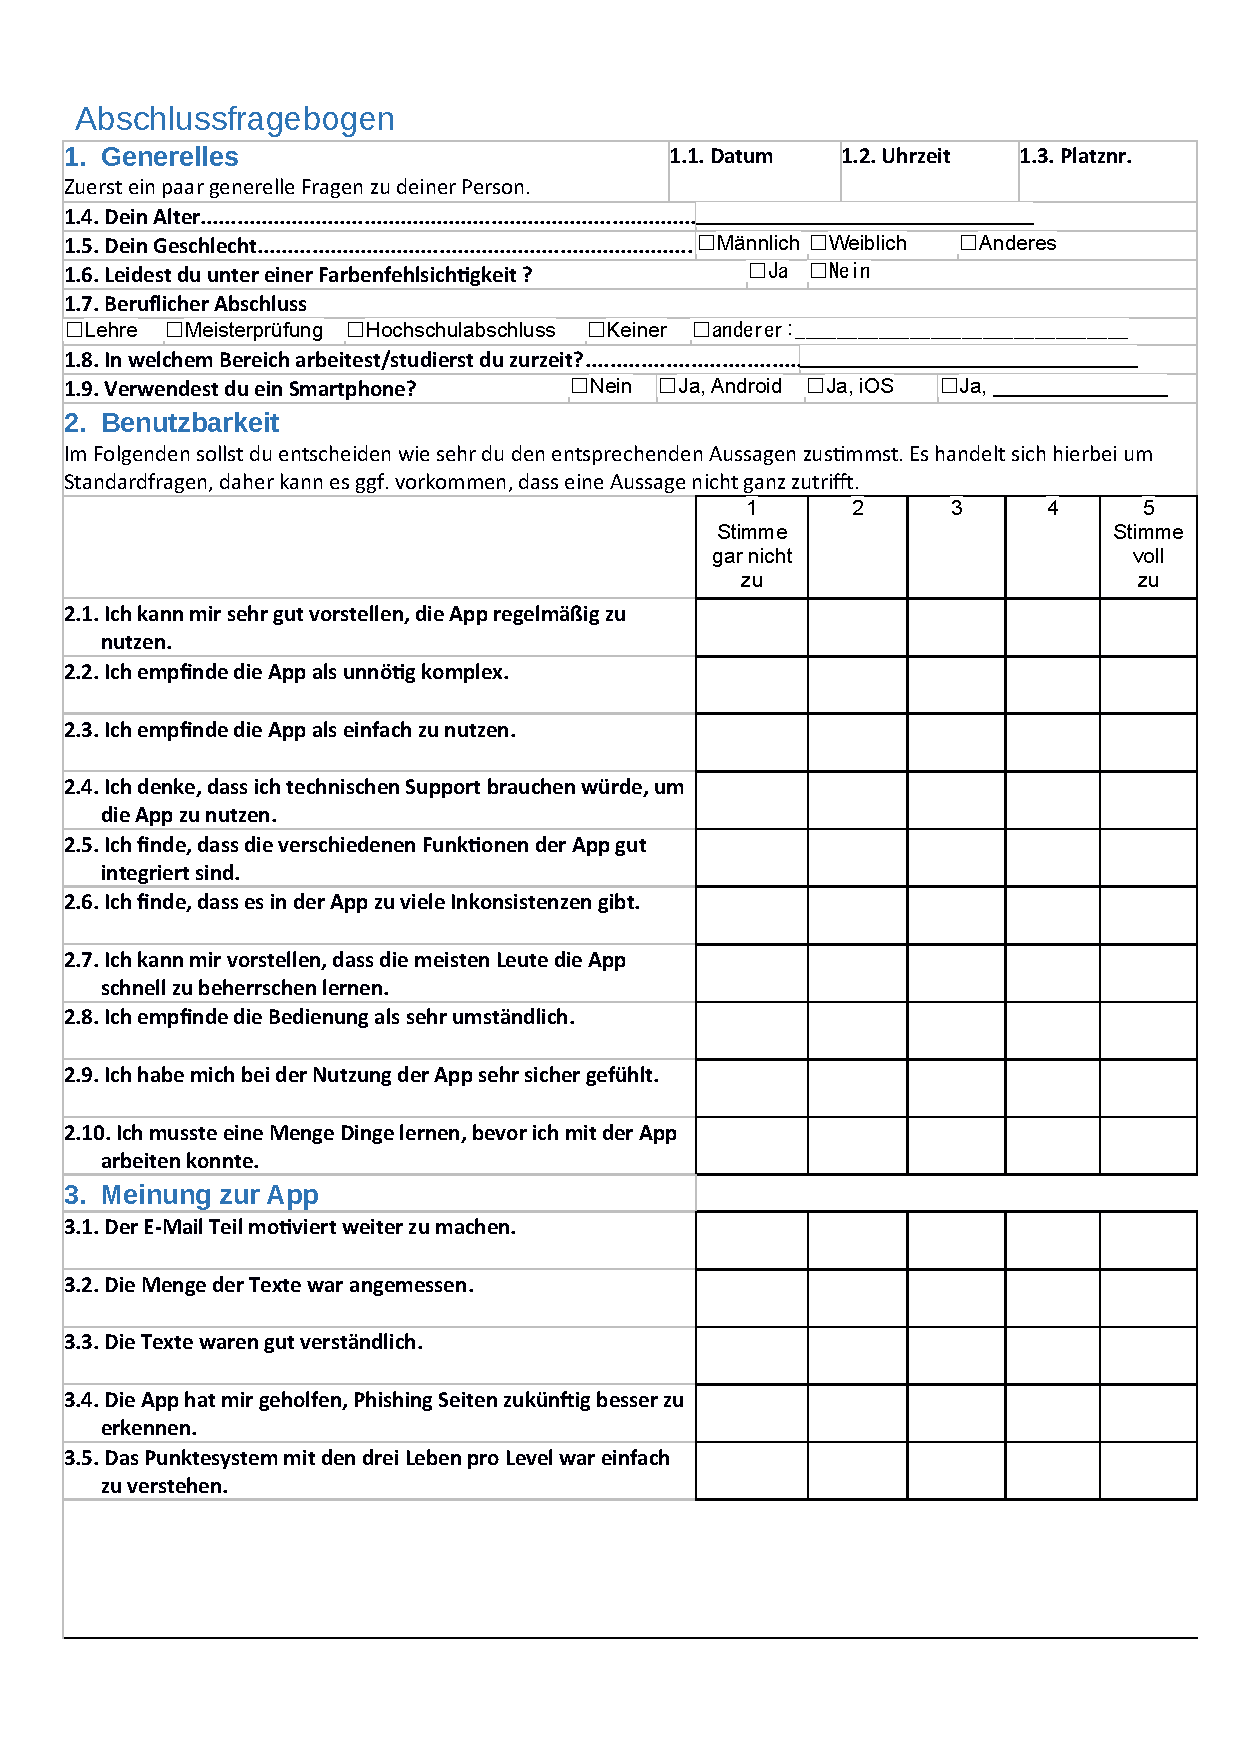
\includepdf[pages={1},frame,scale=0.8]{graphix/after_survey.pdf}

\section{Anti-Phish Certificates for Study Participants}
\label{s:antiphish_certs}


\includepdf[pages={1},frame,scale=0.8]{graphix/zertifikat_gold.pdf}

\includepdf[pages={1},frame,scale=0.8]{graphix/zertifikat_silber.pdf}